\documentclass{article}
\setlength{\parskip}{5pt} % esp. entre parrafos
\setlength{\parindent}{0pt} % esp. al inicio de un parrafo
\usepackage{amsmath} % mates
\usepackage[sort&compress,numbers]{natbib} % referencias
\usepackage{url} % que las URLs se vean lindos
\usepackage[top=25mm,left=20mm,right=20mm,bottom=25mm]{geometry} % margenes
\usepackage{hyperref} % ligas de URLs
\usepackage{graphicx} % poner figuras
\usepackage[spanish]{babel} % otros idiomas
\usepackage[utf8]{inputenc}
\usepackage{wrapfig}
\usepackage{listings}
\usepackage{xcolor}
\usepackage{subfig} 
\definecolor{codegreen}{rgb}{0,0.6,0}
\definecolor{codegray}{rgb}{0.5,0.5,0.5}
\definecolor{codepurple}{rgb}{0.58,0,0.82}
\definecolor{backcolour}{rgb}{0.95,0.95,0.92}
 
\lstdefinestyle{mystyle}{
    backgroundcolor=\color{backcolour},   
    commentstyle=\color{codegreen},
    keywordstyle=\color{magenta},
    numberstyle=\tiny\color{codegray},
    stringstyle=\color{codepurple},
    basicstyle=\footnotesize,
    breakatwhitespace=false,         
    breaklines=true,                 
    captionpos=b,                    
    keepspaces=true,                 
    numbers=left,                    
    numbersep=5pt,                  
    showspaces=false,                
    showstringspaces=false,
    showtabs=false,                  
    tabsize=2
}
\lstset{style=mystyle}
\lstset{language=Python}
\author{Equipo 4 \\Jorge  Fuentes, Tania  Hernandez,
 Anahi Herrera, Gustavo  Díaz, Miriam  Mata, Alejandro Ramos} % author
\title{Práctica 4 \\ Refuerzo del cable de un teleférico} % titulo
\date{\today}

\begin{document} % inicia contenido
\maketitle % cabecera
\begin{abstract} % resumen
\textbf{Objetivo:} El estudiante deberá presentar una propuesta de análisis de formas y de la programación para la ejecución de la optimización (descripción funcional) de características de trabajo especificas que presenta la(s) ventaja(s) (mencionar ventajas). El teleférico es un medio de transporte que consiste en cabinas con capacidad para llevar ungrupo de personas. Estas cabinas viajan suspendidas en el aire transportadas por uno o varioscables. Por ser una estructura poco convencional no se cuenta con un código que norme sudiseño y construcción. Un teleférico debe ser visualizado como sistema estructural en el quesus componentes (anclajes, apoyos, cables) tienen comportamientos diferentes pero que funcionan en conjunto. La línea tiene diferentes componentes, como las pilonas, los balancines y el cable. El cable da nombre a todos los sistemas de transporte por cable, los teleféricos. Los cables de acero están compuestos de hilos de cable que se retuercen alrededor del núcleo del cable. Empresas especializadas fabrican los cables y los montan en el lugar.
\end{abstract}
\newpage
\tableofcontents
\newpage
\section{Introducción}\label{intro} % seccion y etiqueta
El teleférico es un sistema de transporte no tripulado aéreo constituido por cabinas colgadas de una serie de cables que se encargan de hacer avanzar a las unidades a través de las estaciones. Ningún otro elemento como la morfología del terreno es capaz de influir tan claramente en las características de la línea de un teleférico. En consecuencia, es importante el desarrollo de todos los aspectos de los componentes y su correcto funcionamiento, los cuales ofrecen a los pasajeros el máximo confort y seguridad. La línea tiene diferentes componentes, como las pilonas, los balancines y el cable. El cable da nombre a todos los sistemas de transporte por cable, los teleféricos. Los cables de acero están compuestos de hilos de cable que se retuercen alrededor del núcleo del cable. Empresas especializadas fabrican los cables y los montan en el lugar.
%\cite{ff2} CITAR FUENTE

%\begin{figure} % figura
    %\centering
    %\includegraphics[width=150mm]{output3.jpg} % archivo
    %\caption{resultados del programa}
    %\label{grafica}
%\end{figure}
\section{Desarrollo}
\subsection{Nombre y definición de la forma geometría}
\subsubsection{Teleféricos vaivén }
Los teleféricos de vaivén son generalmente bicables y se conocen también como teleféricos pesados o simplemente teleféricos cuando se comparan a telecabinas y telesillas. Son las instalaciones aéreas que permiten mayores vanos superiores a 1 Km\cite{rf1}.\\
Pueden discurrir a gran altura sobre el suelo, permite altura ilimitada si disponen de cabina de evacuación. La capacidad de transporte de estos teleféricos vaivén ronda según la magnitud de la cabina, la velocidad de marcha y la longitud del recorrido entre 500 y 2000 personas/hora.
Las cabinas para este tipo de instalaciones están en constante progresión, tanto en tamaño como en comodidad, seguridad, estética y aerodinámica.

\subsubsection{Cable y sus componentes}
Los cables de acero están constituidos por alambres de acero, generalmente trenzados en hélice (espiral) formando las unidades que se denominan torones (cordones) los cuales posteriormente son cableados alrededor de un centro que puede ser de acero o de fibra. El número de torones (cordones) en el cable puede variar según las propiedades que se desean obtener\cite{rf2}.
\subsubsection{Alcances}
\begin{itemize}
    \item El teleférico funciona con energía eléctrica. Por lo que no emite gases de efecto invernadero ni gases contaminantes como los de los automóviles.
    \item El teleférico funciona con energía eléctrica. Por lo que no emite gases de efecto invernadero ni gases contaminantes como los de los automóviles.
    \item Al ser un sistema aéreo no contamina acústicamente.
    \item Se ha demostrado en estudios que el teleférico puede reducir desde un 15 hasta un 20% de la circulación vehicular en los sectores donde se ha implementado este sistema.
\end{itemize}
El teleférico es una alternativa no tan costosa para mejorar la movilidad urbana de una ciudad. Además de que es un sistema que no contamina con gases o acústicamente.

\subsubsection{Limitaciones} 
Comparte muchas de las tecnologías de los transportes ferroviarios, en especial de los ligeros. Una de las limitaciones que tradicionalmente presentaba este sistema de transporte es la longitud de la línea. Esta no puede ser ilimitada ya que el cable resultaría excesivamente pesado y presentaría problemas de dilatación térmica. Por otro lado, la capacidad de la instalación depende de la longitud. La solución habitual al problema técnico fue el establecimiento de estaciones de transbordo intermedias, con las consiguientes demoras e incomodidades para los viajeros.\\
En la configuración original existían dos secciones, que se han unificado. Para ello se ha dispuesto un segundo cable lastre o contra cable que permite un comportamiento mecánico más estable y un mejor guiado de los vehículos. Esto se complementa con un complejo sistema de tensado de los cables, ubicado en la estación inferior. Esta instalación también puede servir de ejemplo para contemplar las últimas novedades en cuanto a vehículos de funicular. Se incorporan las comodidades que presentan los vehículos recientes de otros modos de transporte, como acceso a discapacitados, aire acondicionado, materiales no deslizantes y anti vandálicos, etc. En estos vehículos se ha llevado al extremo el concepto del viaje como atractivo paisajístico en sí mismo, a pesar de que esa dimensión es menor que en los sistemas aéreos. \\
Otra de las limitaciones que presenta el funicular es la necesidad de que la pendiente de la línea sea aproximadamente constante, dado que los vehículos y las estaciones se adaptan a esa inclinación. Se admite un margen de variación y en parte se puede corregir mediante movimientos de tierra y estructuras, que siempre encarecen la instalación y aumentan el impacto paisajístico. Para disminuir estos problemas y mejorar la comodidad de los pasajeros se están desarrollando vehículos con sistemas hidráulicos que permiten el movimiento de los compartimentos y su adaptación a la pendiente de la línea en cada punto; de este modo el viajero permanece siempre horizontal. \\
En estos momentos ya es posible la explotación completamente automática, reduciendo los costes de personal, manteniendo y un elevado nivel de seguridad. Se trata de una instalación muy controlada en la que no son previsibles incidencias. En ocasiones puede llegar a funcionar de forma similar al ascensor de un edificio\cite{rf3}. 

\begin{figure}[!tbp]
  \centering
  \subfloat[]{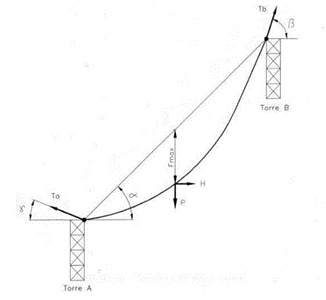
\includegraphics[width=0.4\textwidth]{Imagen1.png}\label{fig:f1}}
  \hfill
  \subfloat[]{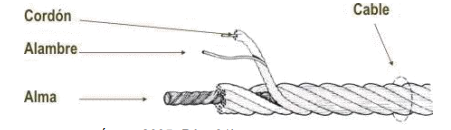
\includegraphics[width=0.4\textwidth]{Imagen2.png}\label{fig:f2}}
  \caption{Diseño de un teleférico}
\end{figure}
\subsection{Estado del arte}
El teleférico es un medio de transporte que consiste en cabinas con capacidad para llevar ungrupo de personas. Estas cabinas viajan suspendidas en el aire transportadas por uno o varioscables. Por ser una estructura poco convencional no se cuenta con un código que norme sudiseño y construcción. Un teleférico debe ser visualizado como sistema estructural en el quesus componentes (anclajes, apoyos, cables) tienen comportamientos diferentes pero que funcionan en conjunto.
\newpage
\subsection{Pasos del desarrollo de la programación}
A continuación, veremos la codificación de la programación en MATLAB.
\begin{lstlisting}
%%%% A 99 LINE TOPOLOGY OPTIMIZATION CODE BY OLE SIGMUND, OCTOBER 1999 %%%
function new_pr42_f(nelx,nely,volfrac,penal,rmin);
% INITIALIZE
x(1:nely,1:nelx) = volfrac;
for ely = 1:nely
  for elx = 1:nelx
      if ely>21
        if elx<31
         passive(ely,elx) = 1;
        else
             passive(ely,elx) = 0;
        end
      end
  end
end
x(find(passive))=0.001;
loop = 0; change = 1.;
% START ITERATION
while change > 0.01
    loop = loop + 1;
    xold = x;
    % FE-ANALYSIS
    [U]=FE(nelx,nely,x,penal);
    % OBJECTIVE FUNCTION AND SENSITIVITY ANALYSIS
    [KE] = lk;
    c = 0.;
    for ely = 1:nely
        for elx = 1:nelx
            n1 = (nely+1)*(elx-1)+ely;
            n2 = (nely+1)* elx +ely;
            dc(ely,elx)=0.;
            for i=1:2
             Ue = U([2*n1-1;2*n1; 2*n2-1;2*n2; 2*n2+1; 2*n2+2; 2*n1+1;2*n1+2],i);
             c = c + x(ely,elx)^penal*Ue'*KE*Ue;
             dc(ely,elx) = dc(ely,elx)-penal*x(ely,elx)^(penal-1)* Ue'*KE*Ue;
            end
        end
    end
    % FILTERING OF SENSITIVITIES
    [dc] = check(nelx,nely,rmin,x,dc);
   % DESIGN UPDATE BY THE OPTIMALITY CRITERIA METHOD
   [x] = OC(nelx,nely,x,volfrac,dc,passive);
   % PRINT RESULTS
   change = max(max(abs(x-xold)));
   disp([' It.: ' sprintf('%4i',loop) ' Obj.: ' sprintf('%10.4f',c) ...
 'Vol.:' sprintf('%6.3f',sum(sum(x))/(nelx*nely)) ...
 ' ch.: ' sprintf('%6.3f',change )])
% PLOT DENSITIES
colormap(gray); imagesc(-x); axis equal; axis tight; axis off;pause(1e-6);
end
%%%%%%%%%% OPTIMALITY CRITERIA UPDATE %%%%%%%%%
function [xnew]=OC(nelx,nely,x,volfrac,dc,passive)
l1 = 0; l2 = 100000; move = 0.2;
while (l2-l1 > 1e-4)
lmid = 0.5*(l2+l1);
xnew = max(0.001,max(x-move,min(1.,min(x+move,x.*sqrt(-dc./lmid)))));
xnew(find(passive))=0.001;
if sum(sum(xnew)) - volfrac*nelx*nely > 0;
l1 = lmid;
else
l2 = lmid;
end
end
%%%%%%%%%% MESH-INDEPENDENCY FILTER %%%%%%%%%%%
function [dcn]=check(nelx,nely,rmin,x,dc)
dcn=zeros(nely,nelx);
for i = 1:nelx
for j = 1:nely
sum=0.0;
for k = max(i-round(rmin),1): min(i+round(rmin),nelx)
for l = max(j-round(rmin),1): min(j+round(rmin), nely)
fac = rmin-sqrt((i-k)^2+(j-l)^2);
sum = sum+max(0,fac);
dcn(j,i) = dcn(j,i) + max(0,fac)*x(l,k)*dc(l,k);
end
end
dcn(j,i) = dcn(j,i)/(x(j,i)*sum);
end
end
%%%%%%%%%% FE-ANALYSIS %%%%%%%%%%%%
function [U]=FE(nelx,nely,x,penal)
[KE] = lk;
K = sparse(2*(nelx+1)*(nely+1), 2*(nelx+1)*(nely+1));
F = sparse(2*(nely+1)*(nelx+1),2); U = sparse(2*(nely+1)*(nelx+1),2);
for ely = 1:nely
for elx = 1:nelx
7
n1 = (nely+1)*(elx-1)+ely;
n2 = (nely+1)* elx +ely;
edof = [2*n1-1; 2*n1; 2*n2-1; 2*n2; 2*n2+1; 2*n2+2;2*n1+1; 2*n1+2];
K(edof,edof) = K(edof,edof) + x(ely,elx)^penal*KE;
end
end
% DEFINE LOADSAND SUPPORTS(HALF MBB-BEAM)
F(40,1) = -1;
fixeddofs = 2*(nely+1):2*(nely+1):2*(nelx+1)*(nely+1);
alldofs = [1:2*(nely+1)*(nelx+1)];
freedofs = setdiff(alldofs,fixeddofs);
% SOLVING
U(freedofs,:) = K(freedofs,freedofs) \F(freedofs,:);
U(fixeddofs,:)= 0;
%%%%%%%%%% ELEMENT STIFFNESS MATRIX %%%%%%%
function [KE]=lk
E = 1.;
nu = 0.3;
k=[ 1/2-nu/6 1/8+nu/8 -1/4-nu/12 -1/8+3*nu/8 ...
-1/4+nu/12 -1/8-nu/8 nu/6 1/8-3*nu/8];
KE = E/(1-nu^2)* [ k(1) k(2) k(3) k(4) k(5) k(6) k(7) k(8)
k(2) k(1) k(8) k(7) k(6) k(5) k(4) k(3)
k(3) k(8) k(1) k(6) k(7) k(4) k(5) k(2)
k(4) k(7) k(6) k(1) k(8) k(3) k(2) k(5)
k(5) k(6) k(7) k(8) k(1) k(2) k(3) k(4)
k(6) k(5) k(4) k(3) k(2) k(1) k(8) k(7)
k(7) k(4) k(5) k(2) k(3) k(8) k(1) k(6)
k(8) k(3) k(2) k(5) k(4) k(7) k(6) k(1)];

%%%% A 99 LINE TOPOLOGY OPTIMIZATION CODE BY OLE SIGMUND, OCTOBER 1999 %%%
function new_pr42_f(nelx,nely,volfrac,penal,rmin);
% INITIALIZE
x(1:nely,1:nelx) = volfrac;
for ely = 1:nely
 for elx = 1:nelx
 if ely>21
 if elx<21
 passive(ely,elx) = 1;
 elseif elx>41
 passive(ely,elx)=1;
 else
 passive(ely,elx) = 0;
 end
 end
 end
end
x(find(passive))=0.001;
loop = 0; change = 1.;
% START ITERATION
while change > 0.01
loop = loop + 1;
xold = x;
% FE-ANALYSIS
[U]=FE(nelx,nely,x,penal);
% OBJECTIVE FUNCTION AND SENSITIVITY ANALYSIS
[KE] = lk;
c = 0.;
for ely = 1:nely
for elx = 1:nelx
n1 = (nely+1)*(elx-1)+ely;
n2 = (nely+1)* elx +ely;
dc(ely,elx)=0.;
for i=1:2
Ue = U([2*n1-1;2*n1; 2*n2-1;2*n2; 2*n2+1; 2*n2+2; 2*n1+1;2*n1+2],i);
c = c + x(ely,elx)^penal*Ue'*KE*Ue;
dc(ely,elx) = dc(ely,elx)-penal*x(ely,elx)^(penal-1)* Ue'*KE*Ue;
end
end
end
% FILTERING OF SENSITIVITIES
[dc] = check(nelx,nely,rmin,x,dc);
% DESIGN UPDATE BY THE OPTIMALITY CRITERIA METHOD
[x] = OC(nelx,nely,x,volfrac,dc,passive);
% PRINT RESULTS
change = max(max(abs(x-xold)));
disp([' It.: ' sprintf('%4i',loop) ' Obj.: ' sprintf('%10.4f',c) ...
 'Vol.:' sprintf('%6.3f',sum(sum(x))/(nelx*nely)) ...
 ' ch.: ' sprintf('%6.3f',change )])
% PLOT DENSITIES
colormap(gray); imagesc(-x); axis equal; axis tight; axis off;pause(1e-6);
end
%%%%%%%%%% OPTIMALITY CRITERIA UPDATE %%%%%%%%%
function [xnew]=OC(nelx,nely,x,volfrac,dc,passive)
l1 = 0; l2 = 100000; move = 0.2;
while (l2-l1 > 1e-4)
lmid = 0.5*(l2+l1);
xnew = max(0.001,max(x-move,min(1.,min(x+move,x.*sqrt(-dc./lmid)))));
xnew(find(passive))=0.001;
if sum(sum(xnew)) - volfrac*nelx*nely > 0;
l1 = lmid;
else
l2 = lmid;
end
end
%%%%%%%%%% MESH-INDEPENDENCY FILTER %%%%%%%%%%%
function [dcn]=check(nelx,nely,rmin,x,dc)
dcn=zeros(nely,nelx);
for i = 1:nelx
for j = 1:nely
sum=0.0;
for k = max(i-round(rmin),1): min(i+round(rmin),nelx)
for l = max(j-round(rmin),1): min(j+round(rmin), nely)
fac = rmin-sqrt((i-k)^2+(j-l)^2);
sum = sum+max(0,fac);
dcn(j,i) = dcn(j,i) + max(0,fac)*x(l,k)*dc(l,k);
end
end
dcn(j,i) = dcn(j,i)/(x(j,i)*sum);
end
end
%%%%%%%%%% FE-ANALYSIS %%%%%%%%%%%%
function [U]=FE(nelx,nely,x,penal)
[KE] = lk;
K = sparse(2*(nelx+1)*(nely+1), 2*(nelx+1)*(nely+1));
F = sparse(2*(nely+1)*(nelx+1),2); U = sparse(2*(nely+1)*(nelx+1),2);
for ely = 1:nely
for elx = 1:nelx
n1 = (nely+1)*(elx-1)+ely;
n2 = (nely+1)* elx +ely;
edof = [2*n1-1; 2*n1; 2*n2-1; 2*n2; 2*n2+1; 2*n2+2;2*n1+1; 2*n1+2];
K(edof,edof) = K(edof,edof) + x(ely,elx)^penal*KE;
end
end
% DEFINE LOADSAND SUPPORTS(HALF MBB-BEAM)
F(40,1) = -1.; F(9760,2)=1.;
fixeddofs = 2*(nely+1):2*(nely+1):2*(nelx+1)*(nely+1);
alldofs = [1:2*(nely+1)*(nelx+1)];
freedofs = setdiff(alldofs,fixeddofs);
% SOLVING
U(freedofs,:) = K(freedofs,freedofs) \F(freedofs,:);
U(fixeddofs,:)= 0;
%%%%%%%%%% ELEMENT STIFFNESS MATRIX %%%%%%%
function [KE]=lk
E = 1.;
nu = 0.3;
k=[ 1/2-nu/6 1/8+nu/8 -1/4-nu/12 -1/8+3*nu/8 ...
-1/4+nu/12 -1/8-nu/8 nu/6 1/8-3*nu/8];
KE = E/(1-nu^2)* [ k(1) k(2) k(3) k(4) k(5) k(6) k(7) k(8)
k(2) k(1) k(8) k(7) k(6) k(5) k(4) k(3)
k(3) k(8) k(1) k(6) k(7) k(4) k(5) k(2)
k(4) k(7) k(6) k(1) k(8) k(3) k(2) k(5)
k(5) k(6) k(7) k(8) k(1) k(2) k(3) k(4)
k(6) k(5) k(4) k(3) k(2) k(1) k(8) k(7)
k(7) k(4) k(5) k(2) k(3) k(8) k(1) k(6)
k(8) k(3) k(2) k(5) k(4) k(7) k(6) k(1)];
\end{lstlisting}
\newpage
\subsection{Resultados de la optimización}
\begin{figure}[htp] % figura
    \centering
    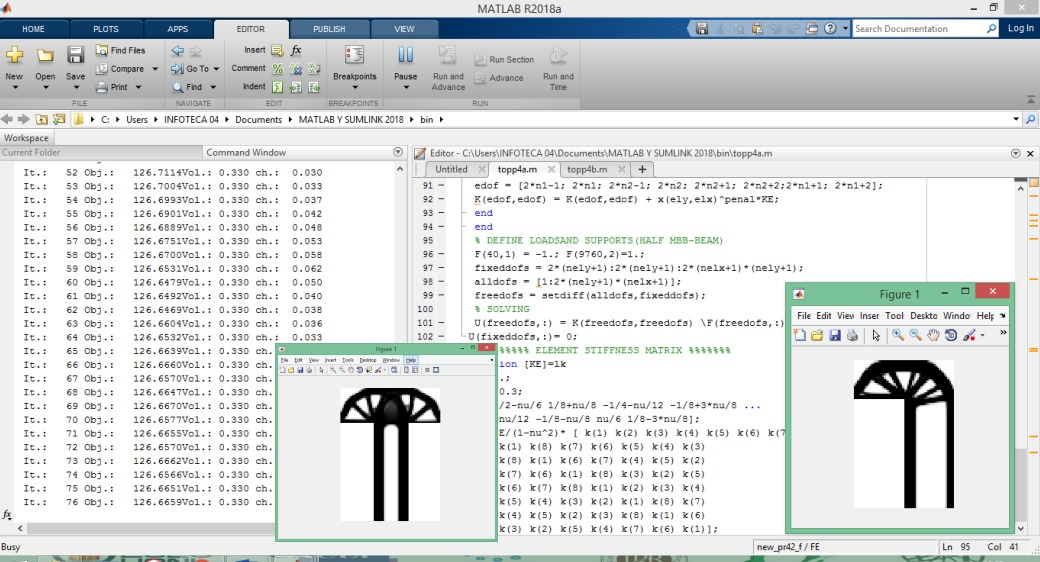
\includegraphics[width=150mm]{Vista completa.jpeg} % archivo
    \caption{Vista completa del resultado.}
    \label{grafica}
\end{figure}
\begin{figure}[!tbp]
  \centering
  \subfloat[]{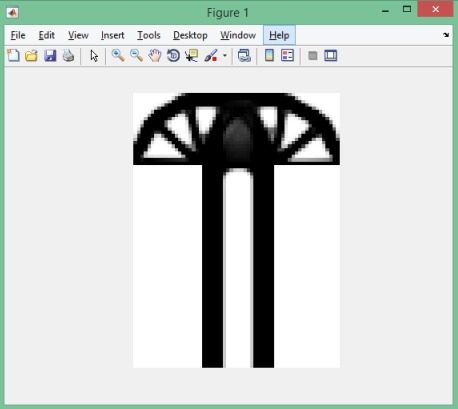
\includegraphics[width=0.4\textwidth]{Vista frontal.jpeg}\label{fig:f1}}
  \hfill
  \subfloat[]{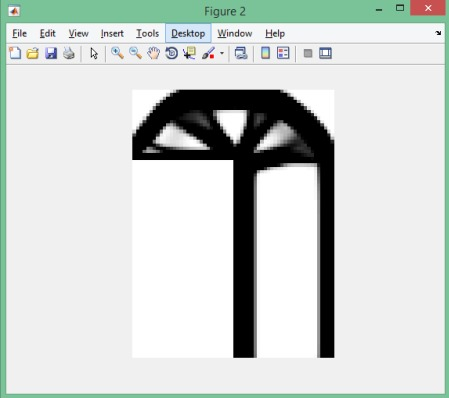
\includegraphics[width=0.4\textwidth]{Vista lateral.jpeg}\label{fig:f2}}
  \caption{Vista frontal y lateral de los resultados.}
\end{figure}
 \newpage
\section{Conclusiones}
\subsection{Jorge  Fuentes}
En esta ocasión tratando de cumplir el objetivo planteado de presentar una propuesta de análisis de formas y de la programación para la ejecución de la optimización de características de trabajo especificas que presenta las ventajas ahora en esta práctica 4 sobre el refuerzo del cable de un teleférico, aplicando los conocimientos previos sobre nuestro dominio en MATLAB así como los pasos de la programación logramos elaborar una estructura de la base de un refuerzo del cable de un teleférico.
\subsection{Tania  Hernandez}
La práctica realizada consistió en la elaboración sobre el refuerzo del cable de un teleférico, para la cual como en todas las anteriores prácticas, se buscó la información respecto a su forma geométrica, estado del arte, etc. Para así pasarnos al resultado final, el cual es sobre el refuerzo del cable de un teleférico en MATLAB.
\subsection{Anahi Herrera}
Para esta actividad se realizaron varias búsquedas de información para ver las características que deben de tener los teleféricos y los aspectos que hay que tener en cuenta para poder construir uno, tanto estudio del terreno como la implementación del tipo de cable correcto para este tipo de transporte. Gracias a todas estas búsquedas y a la implementación correcta de los conocimientos adquiridos pudimos llegar a una realización exitosa de la práctica número cuatro del laboratorio. 
\subsection{Gustavo  Díaz}
Al nosotros conocer un poco mas sobre el funcionamiento de un panorámico/espectacular es más sencillo poder comprender el cómo están hechos para su correcto funcionamiento dado que al ser una estructura que solo se encuentra en soportado por lo que se podría decir un solo punto todas las fuerzas que se genera por sí solo el panorámico y las que se generan por parte de las inclemencias del tiempo hacen que una estructura tan grande tenga diferentes tipos de soportes interiores o externos que lo ayuden a soportar el peso al nosotros hacer la simulación pudimos ver donde es que se concentran la mayoría de los esfuerzos que recaen sobre la estructura y pudimos ver la manera de mejorarla por medio de la optimización.
\subsection{Miriam  Mata}
En el reporte de laboratorio se muestra lo que se realizamos en esta practica, esto usando Matlab, observamos que el tiempo para la realización de ésta fue mayor a la anteriores por el proceso que tuvo que llevar el software para optimizar los esfuerzos, además de ver los espacios en blanco que son elementos pasivos que necesitan ser tomados en cuenta para el diagrama.
\subsection{Alejandro Ramos}
En esta actividad me pareció muy interesante y me puse a investigar cómo se ponen los cables este proceso de la construcción de un teleférico se llama "tirar un cable". Dado que no se puede empezar con el cable pesado y gordo, se tira un cable fino y ligero primero. Aquello se realiza manualmente, con tornos de cable o mediante helicópteros. Pues, se empalme o anuda un cable más gordo y pesado al cable fino y, como consecuencia, se tira mediante un torno de cable. Este proceso se repite con cables cuyo espesor aumenta hasta que haya el cable final con el diámetro correcto en los conjuntos de poleas de las torres. Y me pareció muy importante el saber sobre el refuerzo de los cables.
\bibliography{bib}
\bibliographystyle{plainnat}
\end{document}
